%%==================================================
%% chapter04.tex for SJTU Master Thesis
%% based on CASthesis
%% modified by wei.jianwen@gmail.com
%% version: 0.3a
%% Encoding: UTF-8
%% last update: Dec 5th, 2010
%%==================================================

% \bibliographystyle{sjtu2} %[此处用于每章都生产参考文献]

\chapter{性能评估}
\label{chap:evaluation}

\section{接收信号强度}
\label{sec:rss}

This section presents the experiment and evaluation of on-line and dynamic estimation algorithm proposed previously. Received signal strength measurements, which is implemented by GSM-R network monitoring system, were carried out along the Beijing-Shanghai high-speed railway, and the accuracy and overhead of the algorithm is evaluated in the following.

The measurement experiment is carried out by the Um interface monitoring system of GSM-R networks, as is shown in Fig.~\ref{fig:platform}. The received signal strength was collected along the Beijing-Shanghai high-speed railway, as is shown in Fig.~\ref{fig:experiment}. Since the velocity of train is up to 300km/h and the sampling interval is 500ms limited by the length of measurement multi-frame, it requires repeated data collection to evaluate the estimation algorithm.

%\begin{figure}[!htp]
%%\onelinecaptionsfalse
%\centering
%    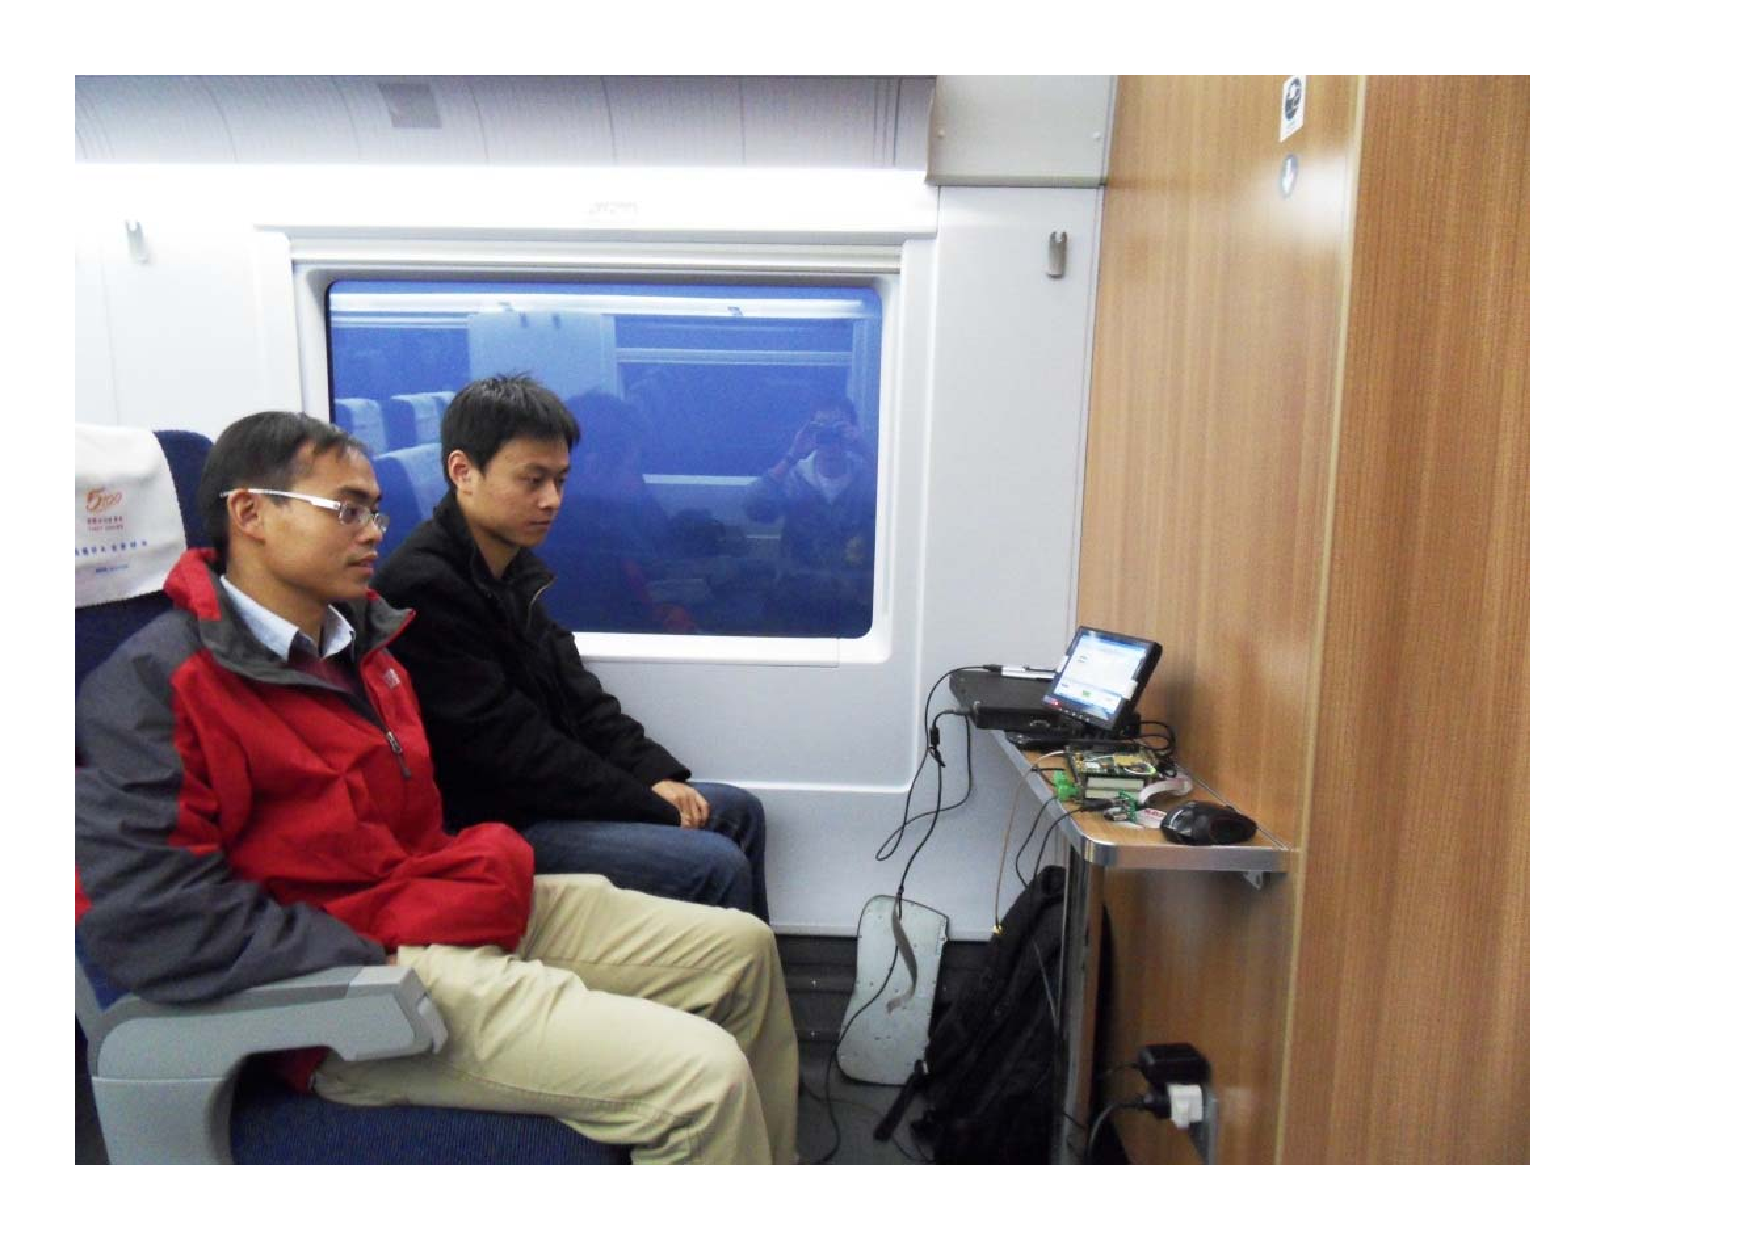
\includegraphics[width=4in]{chap6/test.pdf}
%\bicaption[fig:experiment]{京沪高铁实验测试}{京沪高铁实验测试}{Fig}{Experiment along the Beijing-Shanghai High-Speed Railway}
%\end{figure}

The measurement results is demonstrated in Fig.~\ref{fig:input}, and the long-term and short-term fading are separated after on-line propagation estimation. As is shown in Fig.~\ref{fig:output}, the long-term and short-term fading are differentiated so that they can be analyzed separately. The long-term parts can be used to make propagation prediction by Maximum Likelihood (ML) or Minimum Mean Square Error (MMSE) estimator. On the other hand, the short-term variations are essential to the section of the hysteresis in handoff algorithms.

\begin{figure}[!htp]
\centering
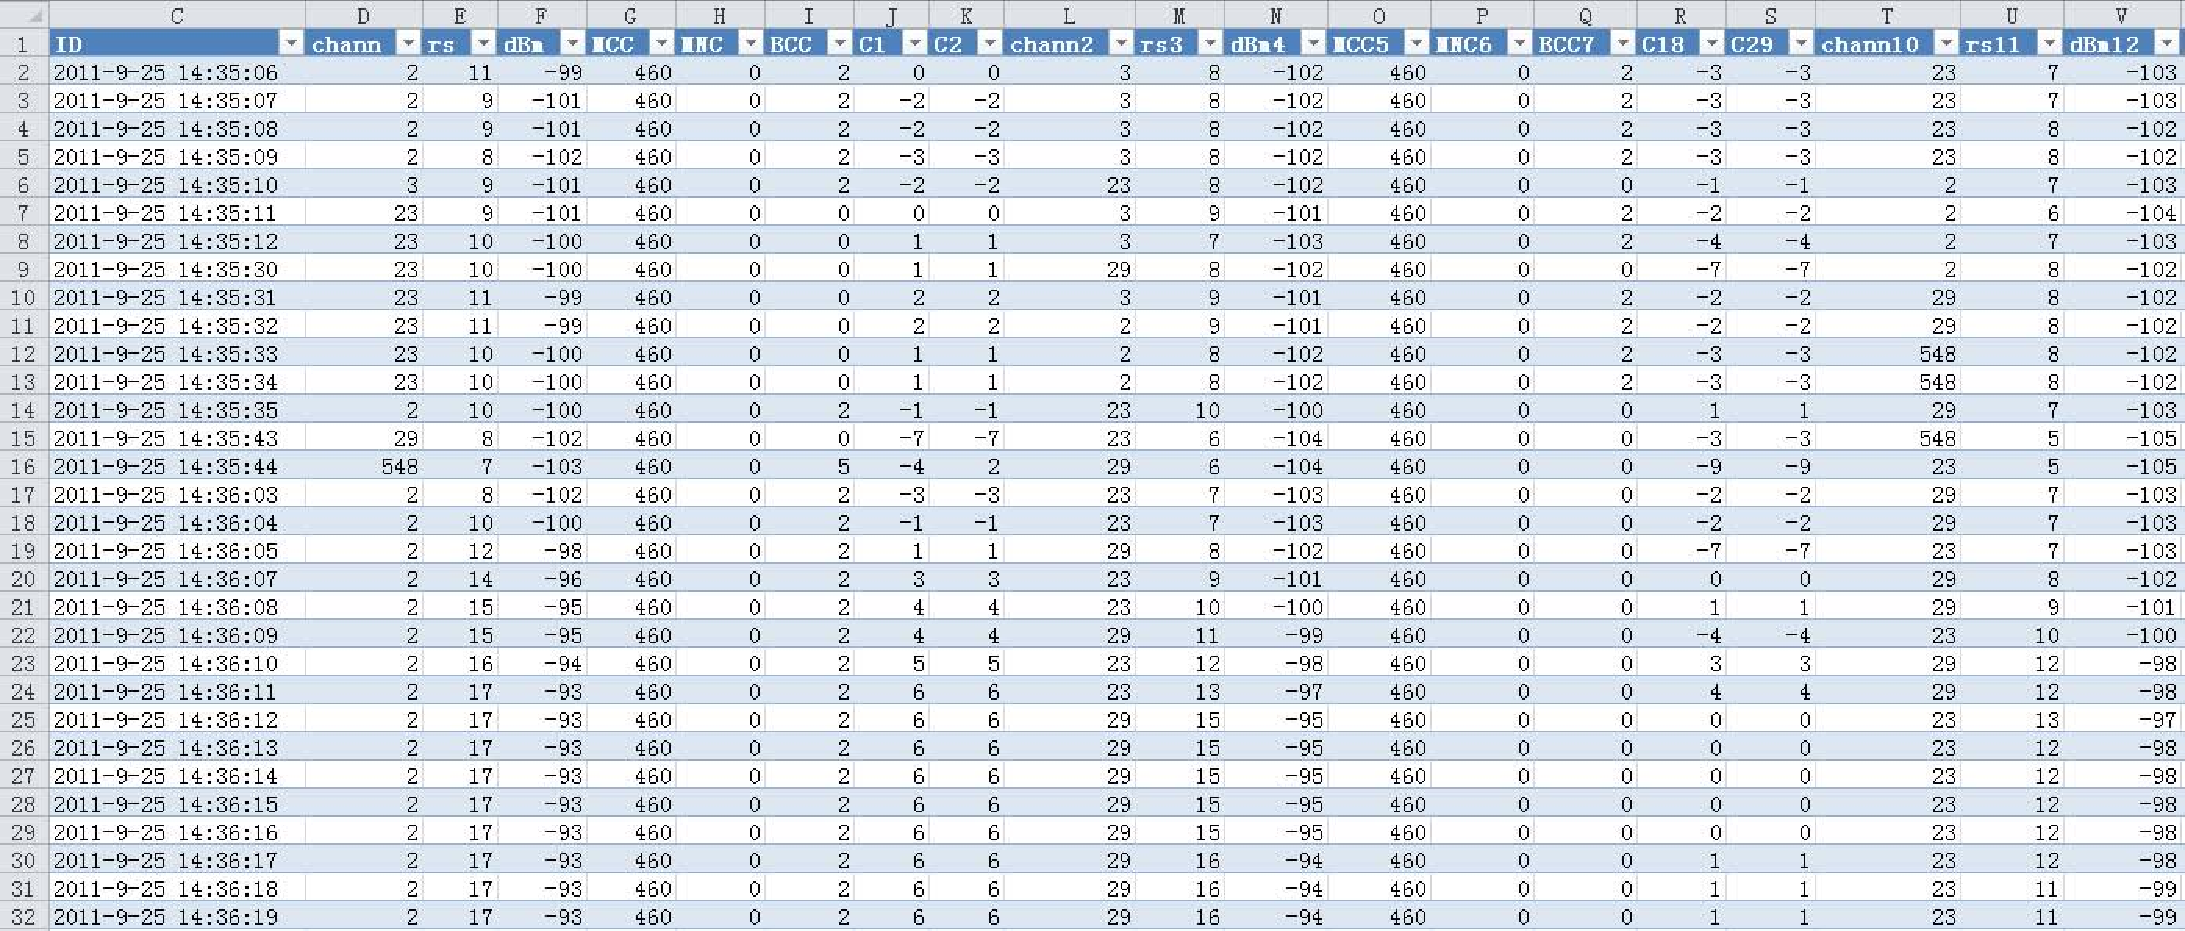
\includegraphics[width=5in]{chap6/xml.pdf}
\bicaption[fig:xml]{信道状态测试结果}{信道状态测试结果}{Fig}{Measurement Results}
\end{figure}

\begin{figure}[!htp]
\centering
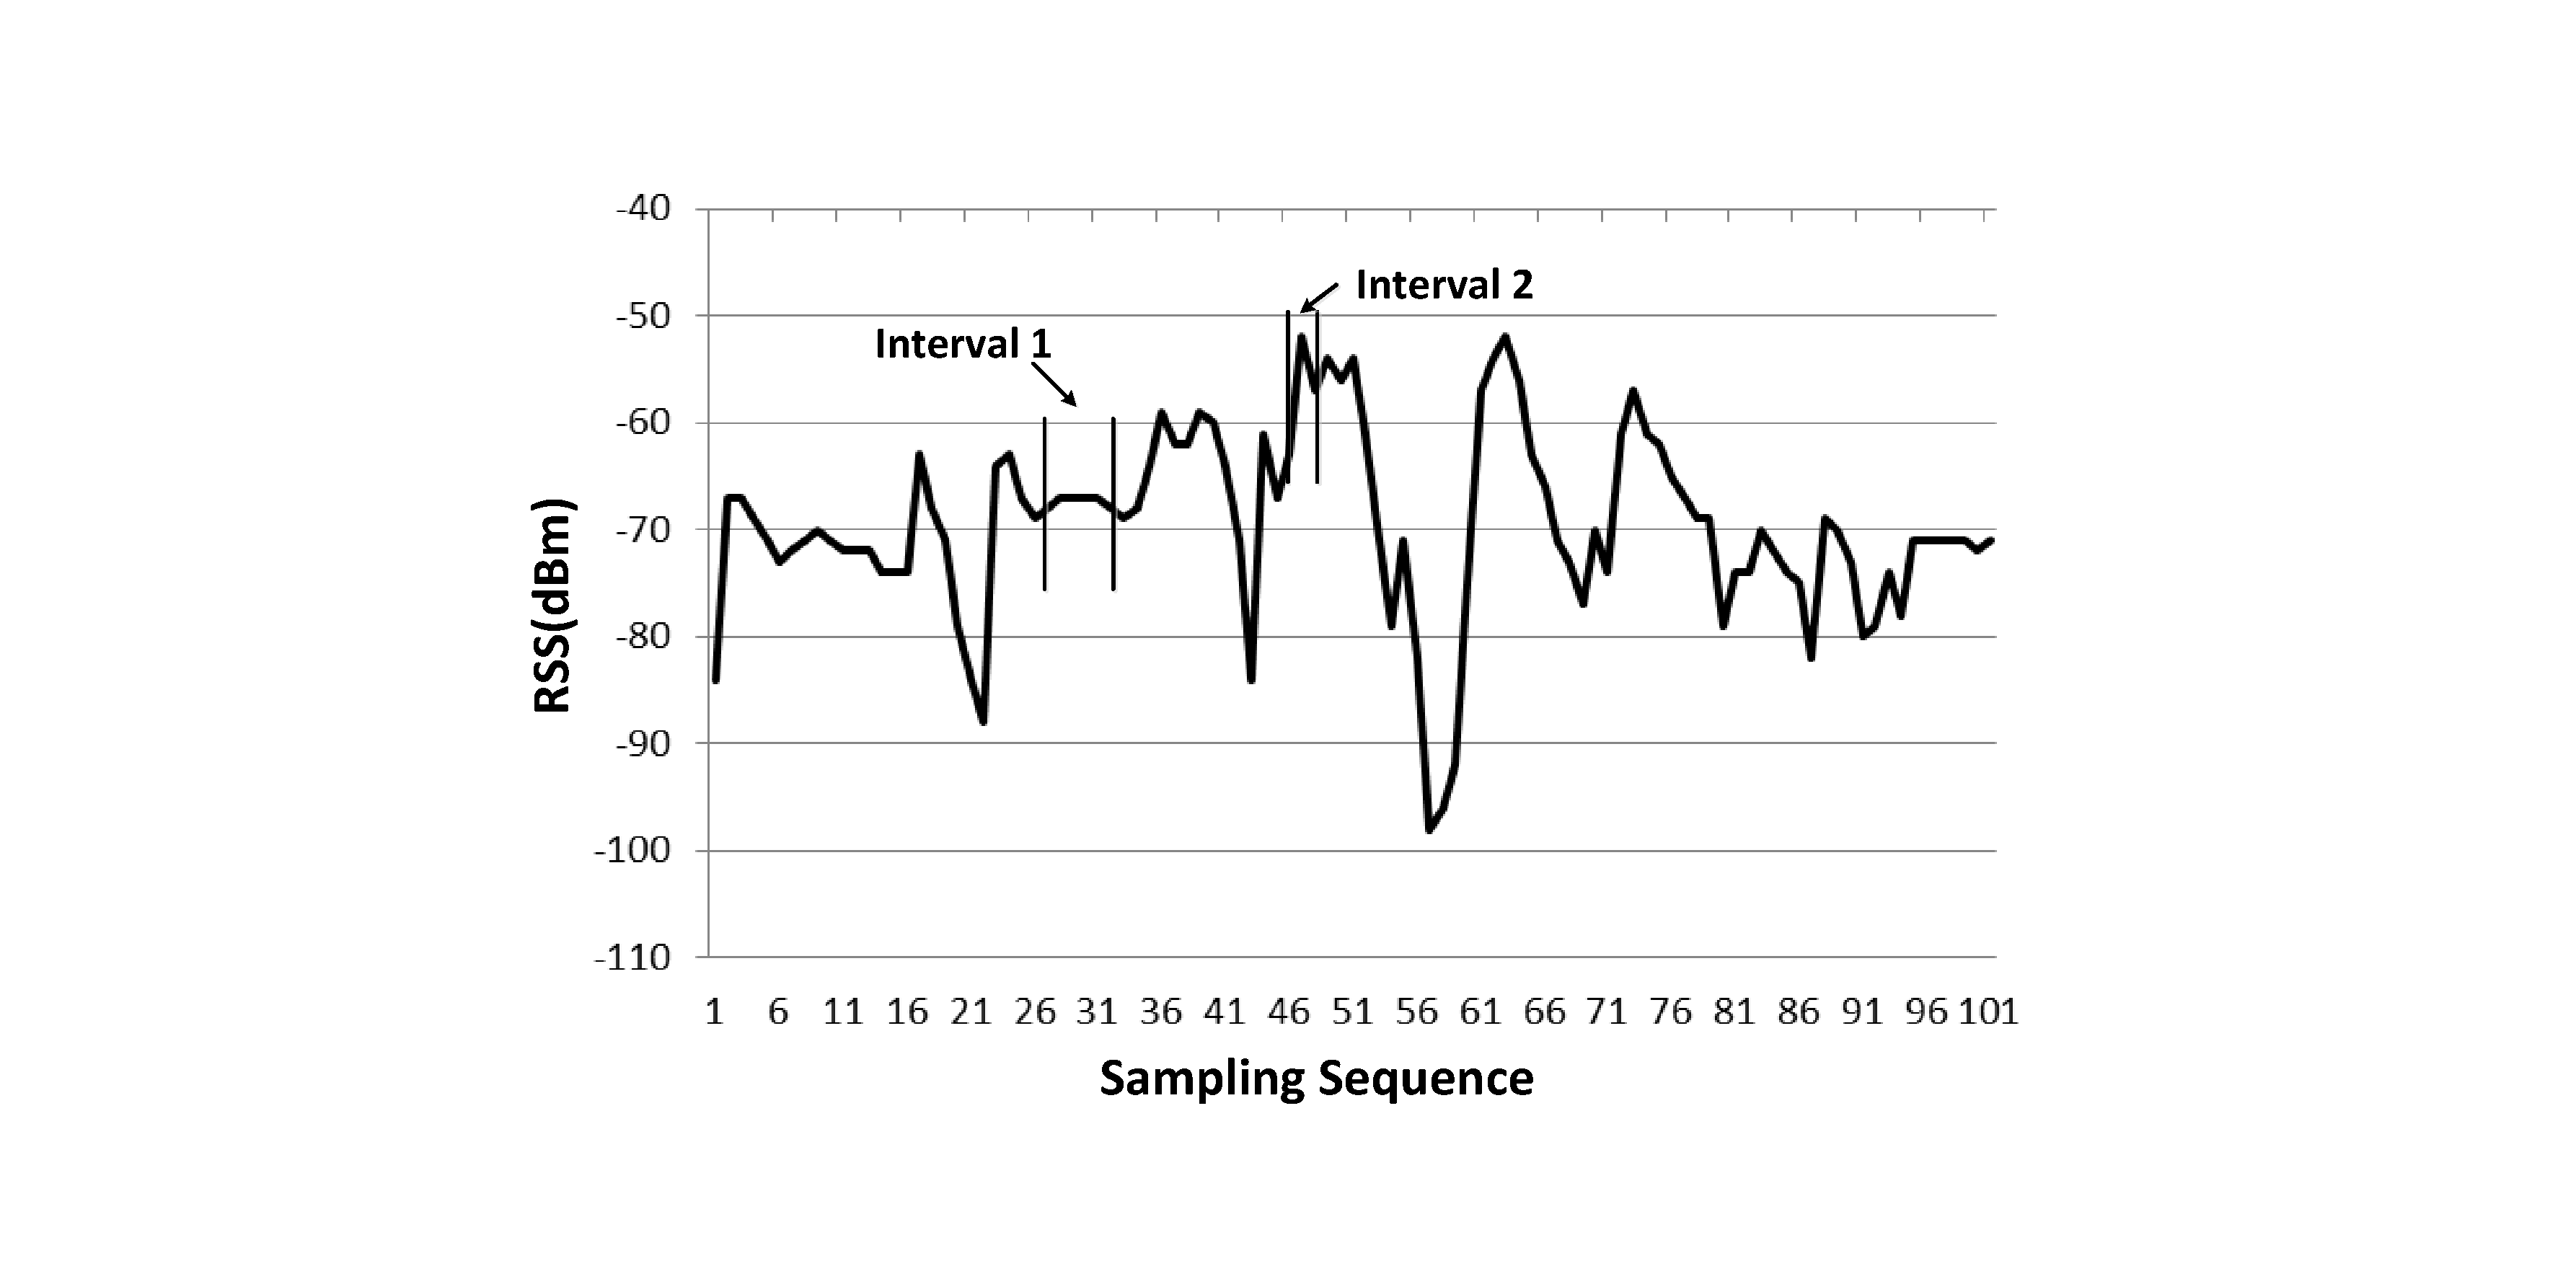
\includegraphics[width=4in]{chap6/result.pdf}
\bicaption[fig:example]{信道状态采样频率}{信道状态采样频率}{Fig}{Example of sampling frequency}
\end{figure}

The estimation results is summarized in Table~\ref{tab:summary} in detail, and it gives the length of statistical interval and number of averaging samples according to propagation environment. The type of different terrain is distinguished by Rician fading factor $K$, it is intensive areas without LOS components when $K=0$, and the propagation environment becomes more flat gradually along with the increase of $K$. The on-line estimating results are compared to Lee's method in the case of $K=0$ which means the fading channels is Rayleigh distributed, and it requires smaller sampling intervals in Lee's method. The power in the direct path increase as the terrain becomes flat, so that the number of averaging samples is less than 5 when $\nu$ becomes larger than 10, and it does not need to make frequent sampling although the length of statistical interval decreases.

%\begin{table}
%\begin{center}
%\caption{Units for Magnetic Properties}
%\label{tb:Units for Magnetic Properties}
%\begin{tabular}{lp{2.5cm}p{4.4cm}}
%\hline\hline
%\rule{-1.9mm}{3.5mm}{Symbol} & {Quantity} & {Conversion from Gaussian and CGS EMU to SI$^\texttt{a}$} \\
%\hline
%\rule{-1.9mm}{3mm}{$\Phi$} & {magnetic flux} & {1 Mx $\rightarrow$ 10$^{-8}$ Wb = 10$^{-8}$ V$\cdot$s} \\
%\rule{-1.9mm}{3mm}{\textit{B}} & {magnetic flux density, magnetic induction} & {1 G $\rightarrow$ 10$^{-4}$ T = 10$^{-4}$ Wb/m$^{2}$} \\
%\rule{-1.9mm}{3mm}{\textit{H}} & \parbox[t]{2.5cm}{\raggedright magnetic field strength} & {1 Oe $\rightarrow$ 10$^{3}$/(4$\pi$) A/m} \\
%\hline
%\hline
%\end{tabular}
%\end{center}
%No vertical lines in table. Statements that serve as captions for the entire table do not need footnote letters.
%
%$^{\texttt{a}}$Gaussian units are the same as cgs emu for magnetostatics; Mx = maxwell, G = gauss, Oe = oersted; Wb = weber, V = volt, s = second, T = tesla, m = meter, A = ampere, J = joule, kg = kilogram, H = henry.
%\end{table}

\begin{table}[!htp]
\renewcommand{\arraystretch}{1}
\bicaption[tab:summary]{信道状态估计结果总结}{信道状态估计结果总结}{Table}{Summary of Experiment Results of Channel State Estimation}
\centering
\begin{threeparttable}[b]
\begin{tabular}{c|c|c|c|c|c|c|c|c|c|c}
%\toprule
\hline
%\cline{1-11}
\multicolumn{1}{c|}{\multirow{3}{*}{Terrain}} & \multicolumn{1}{c|}{\multirow{3}{*}{$K$(dB)}} & \multicolumn{1}{c|}{\multirow{3}{*}{$\nu$}} & \multicolumn{1}{c|}{\multirow{3}{*}{$\sigma$}} & \multicolumn{1}{c|}{\multirow{3}{*}{$2L/\lambda$}} & \multicolumn{1}{c|}{\multirow{3}{*}{$N$}} & \multicolumn{1}{c|}{\multirow{3}{*}{$\Delta d/\lambda$}} & \multicolumn{1}{c|}{\multirow{3}{*}{$\Delta d$(m)}} & \multicolumn{3}{c}{$v_{train}$(km/h)}\\
\cline{9-11}
\multicolumn{1}{c|}{} & \multicolumn{1}{c|}{} & \multicolumn{1}{c|}{} & \multicolumn{1}{c|}{} & \multicolumn{1}{c|}{} & \multicolumn{1}{c|}{} & \multicolumn{1}{c|}{} & \multicolumn{1}{c|}{} & 200 & 250 & 300\\
\cline{9-11}
\multicolumn{1}{c|}{}& \multicolumn{1}{c|}{} & \multicolumn{1}{c|}{} & \multicolumn{1}{c|}{} & \multicolumn{1}{c|}{} & \multicolumn{1}{c|}{} & \multicolumn{1}{c|}{} & \multicolumn{1}{c|}{} & \multicolumn{3}{c}{$\Delta t$(ms)}\\
%\midrule[5pt]
%\hline
%\hline
\cline{1-11}
NLOS\tnote{*}  &  0 &    - & - & 40 & 36 &  1.1 & 0.367 &  2.20 &  1.76 &  1.47\\
\hline
Dense &  0 &   0 & 1 & 55 & 15 &  3.7 & 1.222 &  7.33 &  5.86 &  4.89\\
      &  2 &   4 & 2 & 18 & 12 &  1.5 & 0.500 &  3.00 &  2.40 &  2.00\\
      &  4 & 5.6 & 2 &  9 &  9 &  1.0 & 0.333 &  2.00 &  1.60 &  1.33\\
      &  6 &   6 & 3 & 20 &  7 &  2.9 & 0.967 &  5.80 &  4.64 &  3.87\\
      &  8 &  12 & 3 &  8 &  1 &  8.0 & 2.667 & 16.00 & 12.80 & 10.67\\
Open  & 10 &  18 & 4 & 12 &  1 & 12.0 & 4.000 & 24.00 & 19.20 & 16.00\\
%\bottomrule[10pt]
\hline
%\cline{1-11}
\end{tabular}
\begin{tablenotes}
\item[*] \small Caculated by Lee's method of local mean power estimation in the case of Rayleigh fading
\end{tablenotes}
\end{threeparttable}
\end{table}

\begin{figure}[!htp]
\centering
    \subfigure[接收信号强度与大尺度衰落]{
    \label{fig:input}
    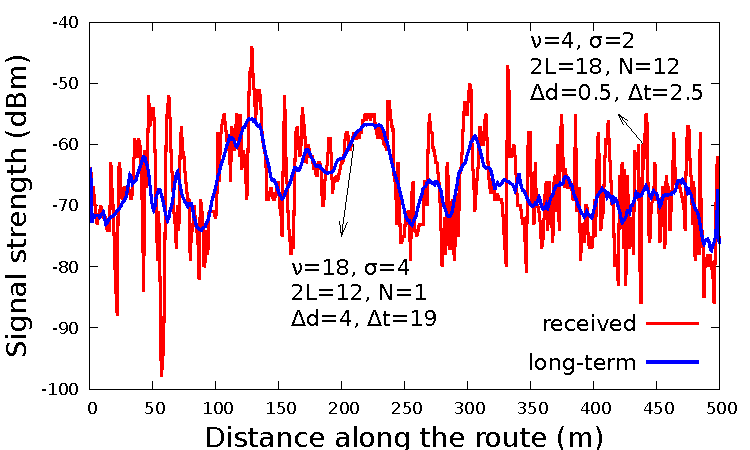
\includegraphics[width=4.5in]{chap6/em.pdf}}
\hspace{1in}
\centering
    \subfigure[小尺度衰落]{
    \label{fig:output}
    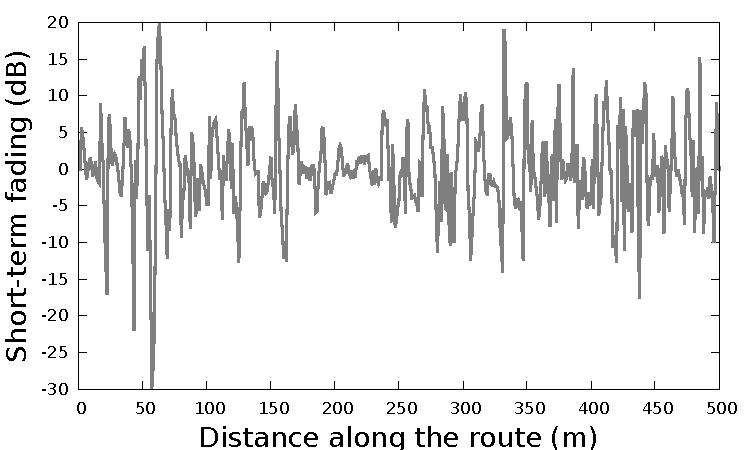
\includegraphics[width=4.5in]{chap6/short.pdf}}
\bicaption[fig:strength]{接收信号强度与信号衰落}{接收信号强度与信号衰落}{Fig}{Received signal strength and signal fading}
\end{figure}

\section{传输成功率}
\label{sec:pdr}

In this section, we first give the accuracy and overhead analysis of DSWA. Then the evaluation of throughput improvements is presented, in which the impact of both DSWA and GradedR are investigated.

For the PDR measurement in static wireless networks, the signal strength is approximately fixed for stationary nodes \cite{reis2006model} and then $p_i$ can be deemed as constant during the averaging process. Since then, $x_i$ is independent and identically distributed random variables, which can be characterized by a Bernoulli process that $\textbf{P(}x_i=1\textbf{)}=p$. When $p_i$ are approximately constant for stationary nodes, both methods can get unbiased estimation of $p_i$. For $p_i=0.8+\sigma$ where $\sigma\sim \textrm{N}(0,0.01)$ is ambient noise, the measured results, whose mean values are 80.23\% and 80.06\% respectively, are both close to the true value of $p_i=0.8$. But DSWA can achieve lower overhead in this case, which will be explained later.

However, in the measurement of realistic networks, EWMA can hardly get sufficient measurement accuracy compared to DSWA. In mobile wireless networks, the propagation environments are complex and communication terminals are on the move particularly, which means the RSS and interference are changing during PDR measurement. This will make the packets received probability $p_i$ changes in short time scale. In this case, it can be characterized by a Generalized Bernoulli process that the probability of $x_i=1$ is different for all values of $i$.
Fig.~\ref{fig:cdf} illustrates the CDF of measurement errors for EWMA and DSWA when applied in mobile scenarios. The measurement errors are within $\pm$0.008 for DSWA, and change from -0.019 to 0.032 for EWMA. The errors of EWMA show that it tends to overestimate the actual PDR, which can also be seen from Fig.~\ref{fig:cdf} that the overall CDF curve of EWMA errors shift to the right of line $Error=0$. Compared with the traditional EWMA method, DSWA can improve the overall measurement accuracy of 89\% higher in mobile scenarios.

\begin{figure}[!htp]
\centering
    \subfigure[CDF of errors]{
    \label{fig:cdf}
    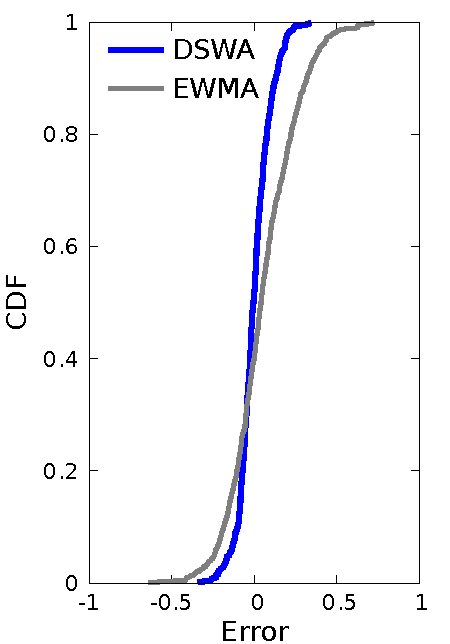
\includegraphics[width=1.5in]{chap6/cdf.pdf}}
    \hspace{1cm}
    \subfigure[Window length and sliding factor of DSWA]{
    \label{fig:overhead}
    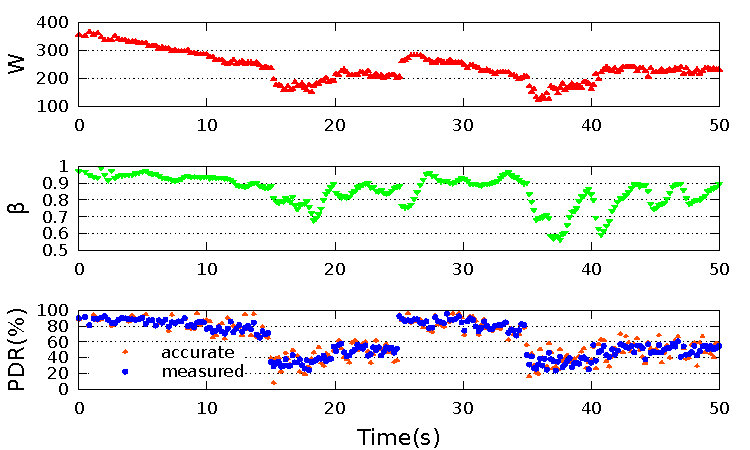
\includegraphics[width=3.5in]{chap6/DSWA.pdf}}
\bicaption[fig:DSWA_error]{传输成功率测试精度与开销}{传输成功率测试精度与开销}{Fig}{Measurement accuracy and overhead for EWMA and DWSA}
\end{figure}

In addition to meet the accuracy requirements, it also deserves attention to reduce measurement overhead, since more sample packets will lower the throughput achieved. The sampling intervals of DSWA are weighted average of last $n$ results so that it can reduce mutations caused by noise and respond quickly to real changes of PDR values. Moreover, the averaging intervals of DSWA are associated with PDR changes to allow a more timely response to sustained decreasing in link quality, and make less frequent samples as network conditions are in steady continuously. Fig.~\ref{fig:overhead} shows an example of DSWA for measuring PDR adaptive to different network conditions. The packet delivery has a sudden decrease at the time of about 15s, and both average interval $W$ and sliding factor $\beta$ drop accordingly. When PDR increases and getting stable from 40s to 50s, $W$ changes from 100 to 200 which will reduce measurement overhead significantly. The average window length of EWMA are approximately constant for certain rate that $W=20$ for 6.5Mbps and $W=500$ for 300Mbps. EWMA can not respond timely when $W=500$ and result in unnecessary errors, especially when there is sudden PDR decline.

\begin{figure}[!htp]
\centering
  \subfigure[1x3]{
  \label{fig:route1}
  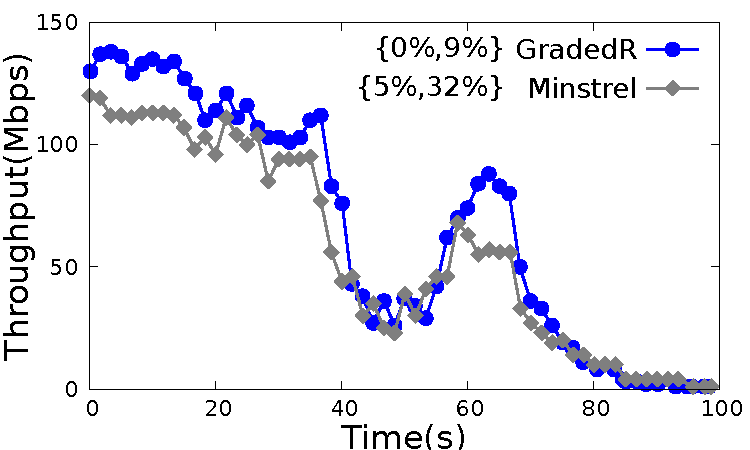
\includegraphics[width=3in]{chap6/route1.pdf}}
  \hspace{1in}
\centering
  \subfigure[2x3]{
  \label{fig:route2}
  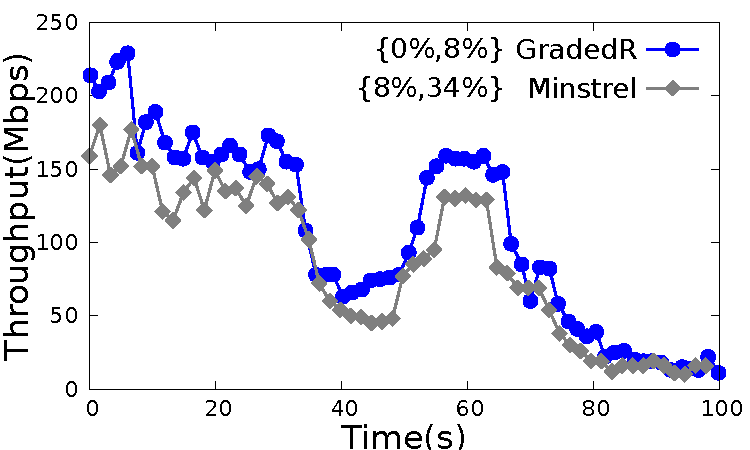
\includegraphics[width=3in]{chap6/route2.pdf}}
  \hspace{1in}
\centering
  \subfigure[3x3]{
  \label{fig:route3}
  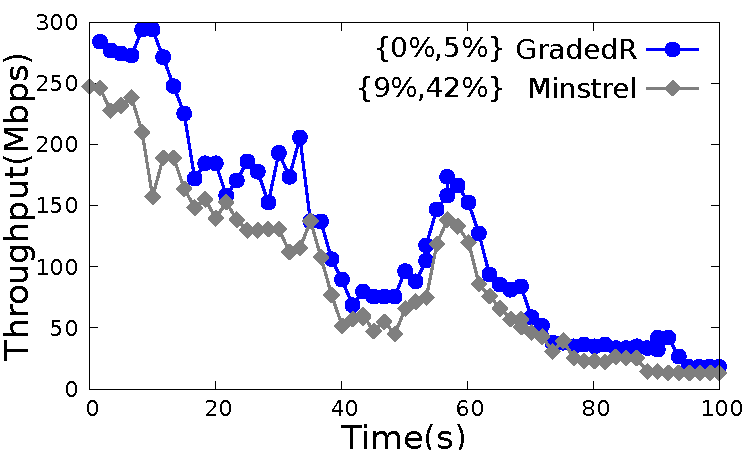
\includegraphics[width=3in]{chap6/route3.pdf}}
\bicaption[fig:route]{吞吐量及传输成功率}{吞吐量及传输成功率}{Fig}{Throughput improvements and PDR results along the route \textbf{r5}}
\end{figure}

\begin{figure}[!htp]
\centering
  \subfigure[1x3]{
  \label{fig:thruput1}
  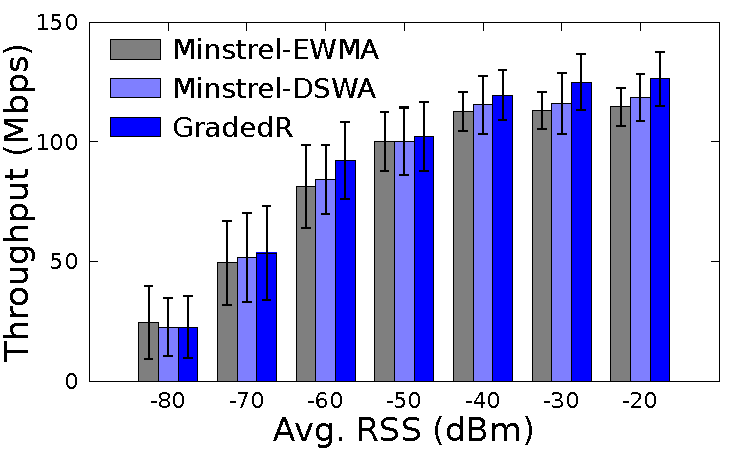
\includegraphics[width=3in]{chap6/goodput1.pdf}}
  \hspace{1in}
\centering
  \subfigure[2x3]{
  \label{fig:thruput2}
  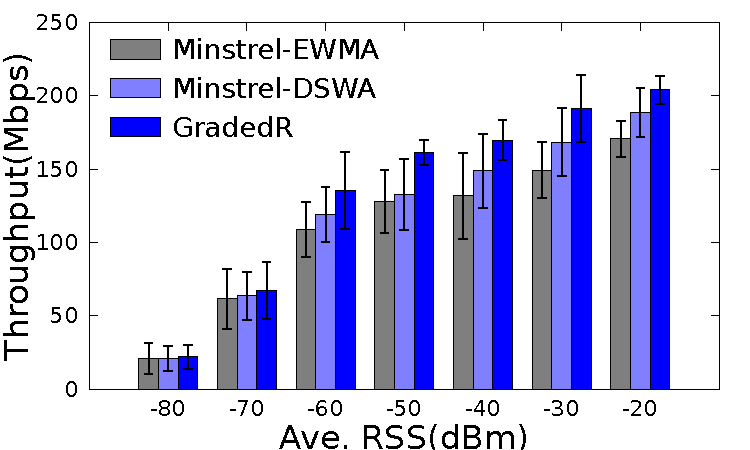
\includegraphics[width=3in]{chap6/goodput2.pdf}}
  \hspace{1in}
\centering
  \subfigure[3x3]{
  \label{fig:thruput3}
  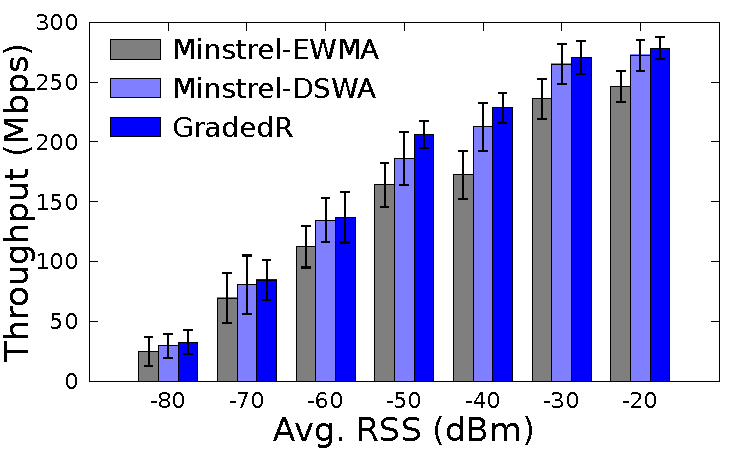
\includegraphics[width=3in]{chap6/goodput3.pdf}}
\bicaption[fig:throughput]{吞吐量及平均接收信号强度关系}{吞吐量及平均接收信号强度关系}{Fig}{Throughput vs. average RSS under different MIMO configurations}
\end{figure}

\section{吞吐量}
\label{sec:throughput}

In order to explore the practical performance improvement of GradedR, mobile experiments are conducted using laptops equipped with above measurement framework. The physical level throughput is taken into account to describe network performance. First, some simple trials are conducted along certain route to verify parameter selection and stability of rate control algorithms. Moreover, the achieved throughput vs. average RSS of different routes are analyzed through statistical calculation. To explore the contributions for throughput improvements of DSWA and GradedR respectively, we also conduct Minstrel rate control with DSWA measurement method. Above approaches are carried out to explore the performance promotions under different MIMO configurations of 1x3, 2x3 and 3x3.

Fig.~\ref{fig:route} illustrates an example of rate control results along the route \textbf{r5} (marked in Fig.~\ref{fig:testbed}) to evaluate the throughput improvement of GradedR of a certain case. The RSS characteristics along this route is given in Fig.~\ref{fig:time}. As is illustrated in Fig.~\ref{fig:route2} of 2x3 MIMO, the throughput is 5-20Mbps higher before the time of 8s, and it will be even more than 30Mbps higher for 3x3 MIMO before 15s in Fig.~\ref{fig:route3}. The reason is that GradedR updates the sensitivity table realtime and chooses the most suitable rate indexes for current conditions rather than randomly select a lower rate. The achieved PDR also has significant impact on throughput. For all the experiments along \textbf{r5}, at least 91\% of PDR values are greater than 90\% for GradedR, but more than 63\% are lower than 90\% for Minstrel. GradedR's rate selection is more smooth and stable, which can avoid concussion of network status, when the network conditions are good enough. And another aspect which will obviously affect the throughput is the measurement overhead. Since Minstrel spends $10\%$ percentage of frames, doing \lq\lq look around\rq\rq~i.e. randomly trying other rates, to gather statistics, the rate being looked around can hardly meet the current situation and it will increase unnecessary load of wireless link. For GradedR, it first adopts DSWA measurement method to get accurate and efficient packet delivery prediction adaptive to network conditions, and then sorts the GradedT to get the parameter configuration according to current PDR and RSS. These two procedures not only reduce the measurement overhead but also improve rate selection efficiency.

The statistical results along route \textbf{r1} to \textbf{r6} is shown in Fig.~\ref{fig:throughput}, and the overall throughput vs. average RSS relationship is evaluated in detail. Generally, GradedR can achieve higher throughput for different MIMO configurations and average RSS values, and the improvements increase with number of spatial streams. The throughput of GradedR is 5-15Mbps higher for 1x3 and 10-40Mbps higher for 3x3 as is shown in Fig.~\ref{fig:thruput1} and \ref{fig:thruput3}. For certain MIMO configuration, the throughput increases are closely related to RSS average value. When the average RSS is less than -60dBm, the throughput of 1 or 2 spatial streams is almost the same, and GradedR is only 5Mbps higher of 3x3 MIMO. The reason for this is that the optional GradedT is limited for less spatial streams and lower average RSS. On the other hand, Minstrel with DSWA can also improve throughput against traditional Minstrel with fixed EWMA. The improvements also increase along with spatial streams and average RSS. As is shown in Fig.~\ref{fig:thruput1}, Minstrel-DSWA can achieve at most 8Mbps higher throughput when RSS is larger than -40dBm for 1x3 MIMO. DSWA can help Minstrel improve throughput of 25/30Mbps for 2x3/3x3 MIMO as RSS is above -40dBm with accurate PDR measurements. The experimental results illustrate that GradedR can achieve throughput gains up to 40\% over Minstrel rate control algorithm under different MIMO configurations, and Minstrel-DSWA can also improve 20\%/25\% higher throughput against Minstrel-EWMA for 2x3/3x3 MIMO.
